%!TEX root = ../main.tex
%%%%%%%%%%%%%%%%%%%%%%%%%%%%%%%%%%
% Links:
%
% Difficulty:
% Companies: 
%%%%%%%%%%%%%%%%%%%%%%%%%%%%%%%%%%


%\begin{figure}
%	\centering
%	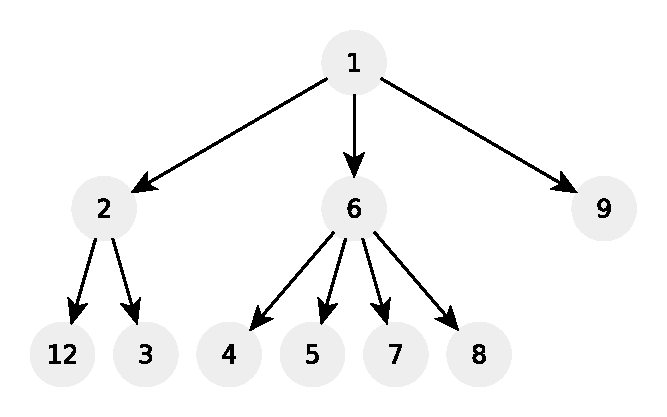
\includegraphics[width=\textwidth]{sources/max_manhattan/images/example1}
%	\caption[Sample short cpation]{Sample Caption}.
%	\label{fig:max_manhattan:example1}
%\end{figure}

\chapter{Max in manhattan neighborhood$^{K}$}
\label{ch:max_manhattan}
\section*{Introduction}
- manahattan disposizione delle strade

\section{Problem statement}
\begin{exercise}
\label{example:max_manhattan:exercice1}
Write a function that given \begin{enumerate*}
	\item a matrix I of $n$ rows and $m$ columns and
	\item  an integer $K > 0$
\end{enumerate*}
returns a new matrix $M$ of size $n \times m$ where $M[i][j]$ contains the maximum value among the elements 
within the manhattan neighborhood of size $K$ for the cell $I[i][j]$.

The Manhattan neighborhood of size $K$ for a cell $(i,j)$ is defined as follows:
\begin{equation}
	N(i,j, K) = \{(p,q) | |i-p|+|j-q| \leq K\}
\end{equation}


%Given a matrix M of size nxm and an integer K, find the maximum element in the K manhattan distance neighbourhood for all elements in nxm matrix.
%In other words, for every element M[i][j] find the maximum element M[p][q] such that abs(i-p)+abs(j-q) <= K.
%Note: Expected time complexity is O(N*N*K)
%Constraints:
%1 <= n <= 300
%1 <= m <= 300
%1 <= K <= 300
%0 <= M[i][j] <= 1000
%Example:
%Input:
%M  = [[1,2,4],[4,5,8]] , K = 2
%Output:
%ans = [[5,8,8],[8,8,8]]
\end{exercise}
	%example1
	\begin{example}
		\label{example:max_manhattan:example1}
		\hfill \\
		Given: $I=
		\begin{bmatrix}
		  1 & 2 & 3  \\
		  4 & 5 & 6  \\
		  7 & 8 & 9  
		\end{bmatrix}
	  $
  and $K=1$ the function return $I=
  \begin{bmatrix}
	  4 & 5 & 6  \\
	  7 & 8 & 9  \\
	  8 & 9 & 9  
	\end{bmatrix}
$
		
	\end{example}

	%example2
	\begin{example}
		\label{example:max_manhattan:example2}
		\hfill \\
		Given: $I=
		\begin{bmatrix}
		  1 & 2 & 3  \\
		  4 & 5 & 6  \\
		  7 & 8 & 9  
		\end{bmatrix}
	  $
  and $K=2$ the function return $I=
  \begin{bmatrix}
	  7 & 8 & 9  \\
	  8 & 9 & 9  \\
	  9 & 9 & 9  
	\end{bmatrix}
$
		
	\end{example}

	\begin{example}
		\hfill \
	
	\label{ex:max_manhattan:example1}
	\end{example}

	\begin{example}
		\hfill \

	\label{ex:max_manhattan:example2}	
	\end{example}



\section{Clarification Questions}

\begin{QandA}
	\item 
	\begin{answered}
		\textit{}
	\end{answered}
	
\end{QandA}

\section{Discussion}
\label{max_manhattan:sec:discussion}
%This problem can be solved easily using dynamic programming.
%DP recurrence:
%dp[k][i][j] = ans. for kth manhattan distance for element (i,j)
%dp[k+1][i][j] = max(dp[k][i-1][j], dp[k][i+1][j], dp[k][i][j-1], dp[k][i][j+1], dp[k][i][j] )
%Recurrence is easy to get once you draw the figure.
%You can optimize by only using N*M*2 space . see solution 2

\subsection{Brute-force}
\label{max_manhattan:sec:bruteforce}

\begin{minipage}{\linewidth}
	\lstinputlisting[language=c++, caption={Sample Caption},label=list:max_manhattan]{sources/max_manhattan/max_manhattan_solution1.cpp}
\end{minipage}

